%\documentclass[preprint]{iucr}
\documentclass{iucr}
 \journalcode{J}
 \papertype{CP}

\usepackage{graphicx}
%\usepackage{minted}

\usepackage[T1]{fontenc}
\usepackage[utf8]{inputenc}

\begin{document}

\title{The Fast Azimuthal Integration Python library}
\shorttitle{PyFAI}

    \author[a]{Giannis}{Ashiotis}
    \author[a]{Aurore}{Deschildre}
    \author[b]{Zubair}{Nawaz}
    \author[a]{Jonathan P.}{Wright}
    \author[a]{Dimitrios}{Karkoulis}
    \author[c]{Fr\'ed\'eric-Emmanuel}{Picca}
    \cauthor[a]{J\'er\^ome}{Kieffer}{jerome.kieffer@esrf.fr}{}
    \aff[a]{European Synchrotron Radiation Facility, 71 Avenue
    des Martyrs, 38000 \city{Grenoble},
    \country{France}}
    \aff[b]{SESAME, P.O. Box 7, \city{Allan} 19252, \country{Jordan}}
    \aff[c]{Synchrotron Soleil, L'Orme des Merisiers, 91190 \city{Saint-Aubin},
    \country{France}}
    \shortauthor{Kieffer et al.}

\keyword{Powder diffraction}
\keyword{small-angle X-ray scattering}
\keyword{geometry calibration}
\keyword{data reduction}
\keyword{image analysis}
\keyword{GPU programming}
\keyword{Python}

\maketitle

\begin{synopsis}
Details the geometry, peak-picking, calibration and integration procedures
on multi- and many-core devices implemented in the Python library for high
performance azimuthal integration.
\end{synopsis}

\begin{abstract}
PyFAI is an open source software package designed to perform azimuthal and
radial integration and, correspondingly, 2D regrouping on area detector frames for small and wide
angle X-ray scattering experiments.
It is written in Python (with binary sub-modules for performances), a
language widely accepted and used by the scientific community today, which enables
the users to easily incorporate the pyFAI library into their processing pipeline.
This work focuses on recent work, especially the ease of
calibration, its accuracy and the execution speed for integration.
\end{abstract}

\section{Introduction}

Azimuthal integration is a common mathematical operation when using area
detectors for recording powder diffraction and scattering patterns, which
ensure larger solid angle coverage and hence a better harvest of X­-ray photons.
This data reduction step is often one of the most time ­consuming tasks in the
processing pipeline and limits sometimes the productivity of modern synchrotron
beamlines, where diffraction is used to probe samples with a point-focused
beam in 2D raster scans or diffraction tomography experiments using
detectors capable of high framerates.

We describe the version 0.10 of the Python library pyFAI 
(released in October 2014) which is designed for such data reduction processing,
including pre-processing, image re-binning (geometry distortion, 1D and 2D
averaging) and the auxiliary tools\cite{pyfai}. 
Among these tools, we will focus on the one used to
calibrate the experimental setup of a powder diffraction  
or SAXS experiment (that comprises
an area detector) by exploiting the Debye-Scherrer rings collected from a
reference compound.
After describing how the experimental geometry is internally represented in
pyFAI, the various image analysis algorithms used to extract Debye-Scherrer
rings are presented.
The peak positions are combined with the prior knowledge of a calibrant
(d-spacing) and the wavelength of the X-rays  to refine of the detector's position in space.

Once this geometry is known, azimuthal regrouping can be performed after
typical corrections are done: dark-current subtraction, flat-field,
solid-angle and polarization correction are included in the standard processing
pipeline.
PyFAI implements various integration algorithms, including
multiple pixel splitting schemes, which will be described and mutually compared
based on speed, accuracy and memory consumption.
An example will be given on how pyFAI can be used to decompose
diffraction images into amorphous and crystalline components and how this can be
applied to serial crystallography.

As pyFAI is a library, other projects related to pyFAI have been created and
will be briefly described, most of them providing integrated
graphical user interfaces (GUI).
Appendices contain information about the pyFAI project structure, an
overview on how to calibrate the experimental setup parameters as well as
a description of how the many-core azimuthal integration is implemented using
OpenCL \cite{opencl}.

\section{Experimental geometry}

In pyFAI, the basic configuration is defined by the description of an
area-detector whose position in space is determined through the sample
position and the incident X-ray beam.

\subsection{Detector}
Like most other diffraction image processing packages, pyFAI allows the definition of
2D detectors with a constant pixel size (in metre), but this approach reaches
its limits with several detector types, such as multi-module and fibre optic
taper coupled detectors.
Large area pixel detectors are often composed of smaller modules (i.e. Pilatus
from Dectris, Maxipix from ESRF,
\ldots).
By construction, such detectors exhibit gaps between modules along with
pixels of various sizes within a single module, hence they require specific
data masks.
Optically coupled detectors need also to be corrected
for small spatial displacements, often called geometric distortion.
This is why detectors need more complex descriptions than just the pixel size.
To avoid complicated and error-prone sets of parameters, detector classes have
been introduced.

\subsubsection{Detectors classes} are used to define families of detectors.
In order to take the specificities of each detector into account, pyFAI
contains about 40 detector classes. These contain a mask
(invalid pixels, gaps, \ldots) and a method to calculate the pixel positions in Cartesian
coordinates.
For optically coupled CCD detectors, the geometrical distortion is often
described by a bi-dimensional cubic spline which can be imported into
the detector instance and used to calculate the actual pixel position in space.

\subsubsection{Nexus Detectors:}
Any detector object in pyFAI can be saved into a HDF5 file following the NeXus
convention \cite{nexus}\footnote{slightly extended as pyFAI's detector
definition is richer than the one provided by the NIAC}.
Detector objects can subsequently be restored from the disk, making
complex detector definitions that are meant to be error-prone.
Pixels of an area detector are saved as a 4D dataset: i.e. a 2D
array of vertices pointing to every corner of each pixel, generating
an array of shape: ($Ny$, $Nx$, $Nc$, 3) where $Nx$ and $Ny$ are the dimensions of the
detector, $Nc$ is the number of corners of each pixel, usually 4, and the last
entry contains the coordinates of the vertex itself.
This kind of definition, while relying on large description files,
can address some of the most complex detector layouts:
\begin{itemize}
  \item hexagonal pixels (i.e. Pixirad detectors)
  \item curved/bent imaging plates (i.e. Rigaku)
  \item pixel detectors with tiled modules  (i.e. some Xpad detectors from
  ImXpad)
  \item semi-cylindrical pixel detectors (i.e. Pilatus12M from Dectris).
\end{itemize}

\subsection{Geometry}
In pyFAI, the experiment geometry is determined by the position of the
detector in space, the origin being located at the sample position, more precisely where the
X-ray beam crosses the diffractometer main axis.
The detector being a rigid body, its position in space is described by
six parameters: 3 coordinates and 3 rotations (figure \ref{PONI}).
In pyFAI, the beam centre is not directly used as it is ill-defined with
highly tilted detectors.
Like SPD \cite{spd}, we use the orthogonal projection of the origin on
the detector surface called PONI (for Point Of Normal Incidence).
For non planar detectors, the PONI is defined in the plane $d3=0$ in
the detector's coordinate system.
The sample-to-detector distance is defined as the origin$-$PONI distance
(abbreviated \textit{dist}) and the PONI coordinates (abbreviated
\textit{poni1} and \textit{poni2}) are measured in the detector's reference
system (origin at the lower left corner of the image, looking from the
viewpoint of the sample).
As the pixel size may not be constant, all 3 distances (\textit{dist},
\textit{poni1} and \textit{poni2}) are given in metre.
The 3 rotations (named \textit{rot1}, \textit{rot2} and \textit{rot3} in
radians)
correspond to the rotations along the three orthogonal axes around the origin
(sample position) in this order:
vertical axis, horizontal axis and finally along the beam axis.

\begin{figure}
\label{PONI}
\begin{center}
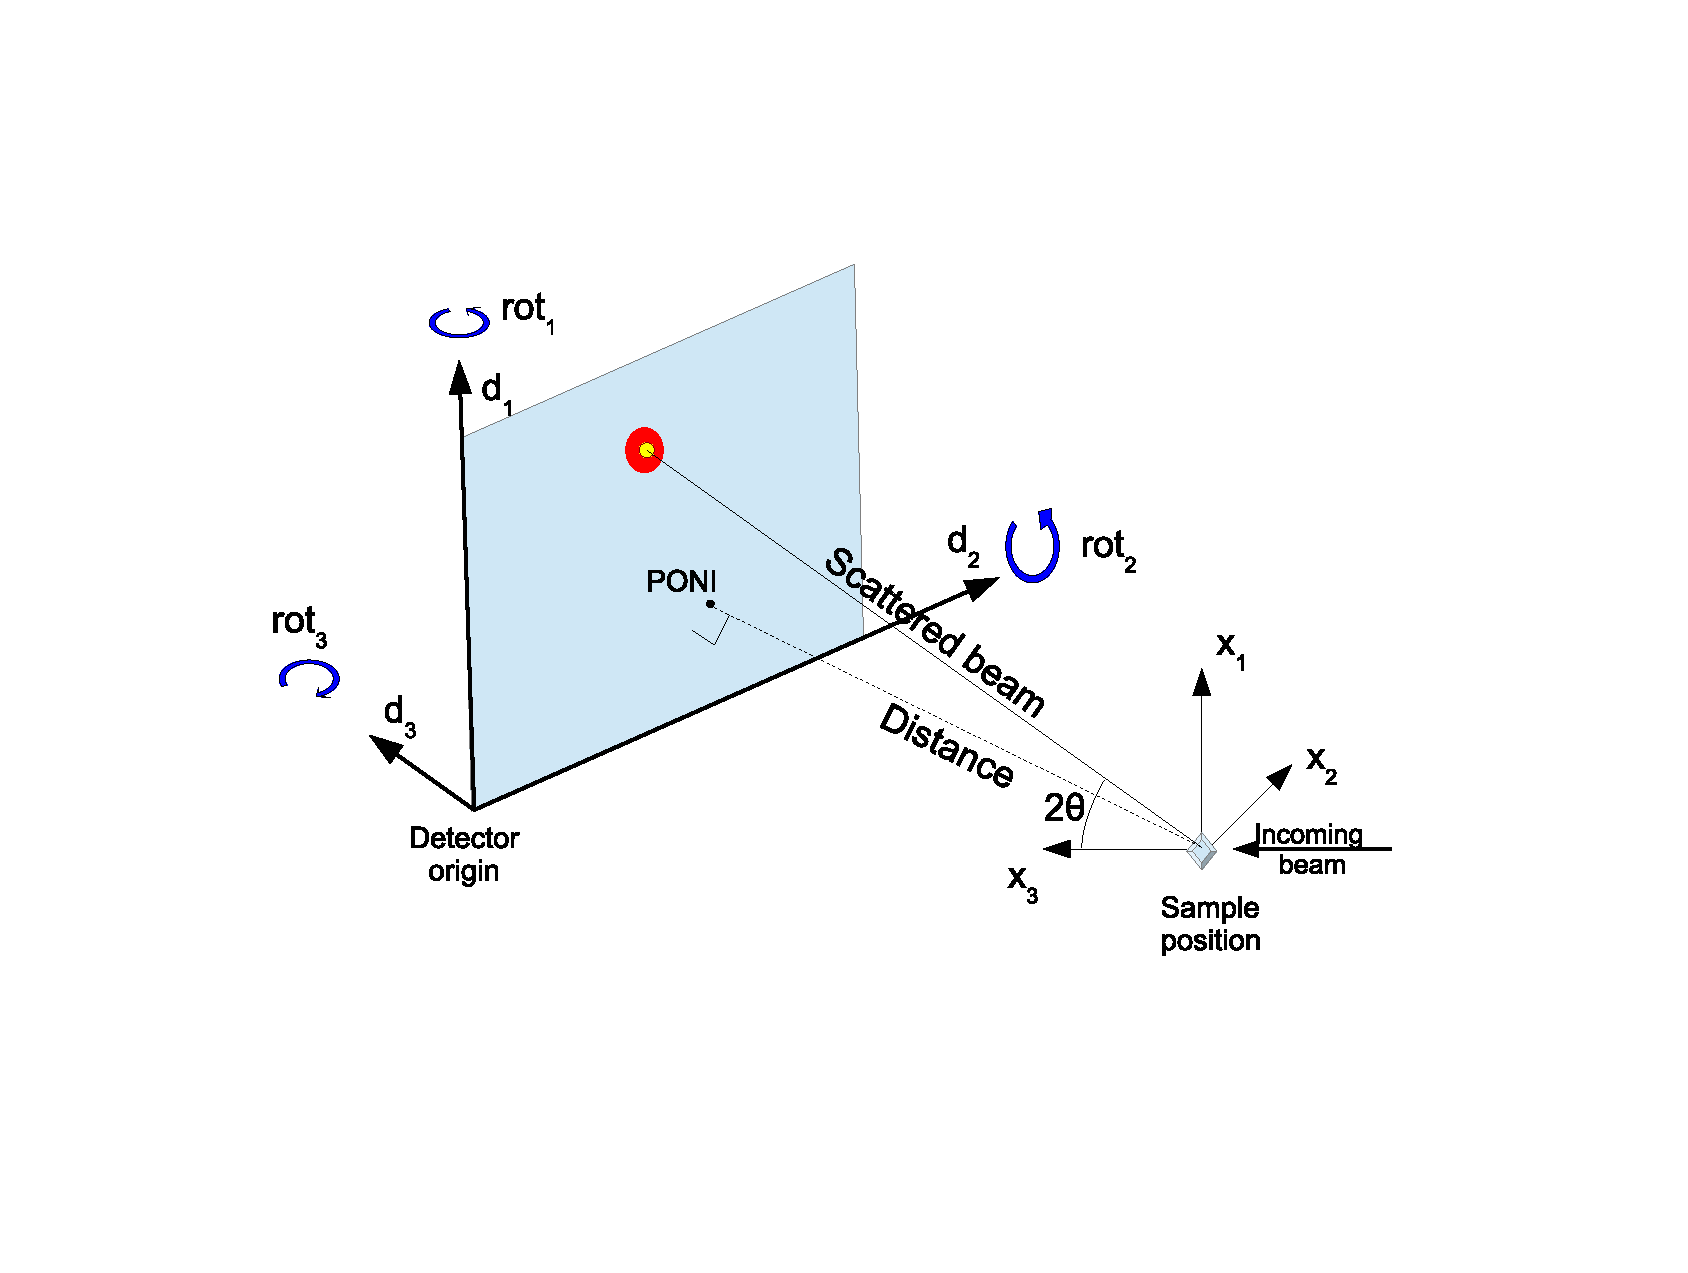
\includegraphics[width=9cm]{PONI.eps}
\caption{The geometry used by pyFAI is inspired by SPD \cite{spd}.}
\end{center}
\end{figure}

When all rotations are zero, the detector is in transmission mode with the
incident beam orthogonal to the detector's surface.
The choice of S.I. units may look cumbersome or odd to users familiar
with other tools like FIT2D \cite{fit2d} or SPD \cite{spd}.
To address such issues, the geometry used in pyFAI can be
exported to and imported from parameter sets compatible with other software
packages.
Geometries used in other codes can be promptly included in pyFAI to ease
comparison of results and cross-validation of approaches.

\subsubsection{Binning}
One of the strengths of the above geometry is the capability of performing
binning operations on the detector without having to re-calibrate or
re-calculate the position in space.
All pyFAI detector classes have a binning option available that can increase the
pixel size and divide the detector shape accordingly.
This works even for detectors that require distortion correction: pyFAI can bin
or un-bin the spline describing the distortion, on the fly, the position of the
PONI being independent of the pixel coordinates.

\section{Calibration}

The calibration of the detector position is performed using the Debye-Scherrer
rings collected from a reference powder called \textit{calibrant}.
The rings are extracted (see \ref{massif}) and control points are placed at the
local maxima on the rings.
The geometry of the experiment is obtained from a least squares fitting of
the $2\theta$ angles.
In this work we will call them ``rings'' even if, for planar detector,
they are actually the conic intersections of the X-ray beam cones
with the detector plane.
PyFAI does not assume that rings are conic sections (the detector could
be non planar) and is able to optimize the
geometric parameters of a wide range of experiments.
The support for the geometry refinement of non-planar detectors is still under
development.

\subsection{Calibrant}
PyFAI provides ten calibrant descriptions covering the most used ones: ceria,
corundum, gold, lanthanum hexaboride and silicon for powder diffraction
measurements; silver behenate, tetradecanol and para-bromobenzoic acid for small
angle scattering experiments.
Any file containing $d$-spacing values in angstrom can be used as calibrant and
loaded into the \textit{Calibrant} class.
The \textit{calibrant} object is in charge of
calculating the reference aperture of the diffraction cones ($2\theta$),
provided the wavelength or energy is known.

\subsection{Peak-picking}
With the advent of micro- and nano-focused beams at modern synchrotron
facilities \cite{id13}, fewer crystals get hit by the beam going through the
sample causing the Debye-Scherrer rings to be spotty.
As grinding reference powder is not advised (it would broaden the peaks
and may even introduce strain), we decided to
address this issue by further analysing and reconstructing the Debye-Scherrer rings.
An alternative approach would be the use of single crystal indexation techniques, using
for example the Fable software \cite{fable} as demonstrated for diffraction
tomography experiments \cite{bonnin}.

\subsubsection{``Massif'' extraction}
\label{massif}
allows a clear separation between regions containing high
photon counts (rings) and background.
This is done by calculating the difference between the image and a blurred version
of the same image, using a Gaussian blur filter (of a width $\sigma$).
The borders of high intensity regions (called \textit{massif}) feature
negative intensities in the difference image, so positive regions are labelled
as (fractions of) a ring.
Peaks, i.e. local maxima,
are sampled within the same region and belong to the same ring.
The width of the Gaussian, $\sigma$, in pixel units, has to be larger than the
typical distance between two peaks within a ring and smaller than the distance between two
rings.
PyFAI takes heuristic approach to guess an acceptable parameter value in
most cases, while providing also a manual override through the command line
argument ``\textit{-\,-gaussian=$sigma$}''.

\subsubsection{Sub-pixel accuracy}
\label{subpixel}
is often needed when measuring strains in materials, as highlighted in
\cite{to5079}.
The accuracy on the peak position is obtained using a second order Taylor
polynomial of the intensity in the neighborhood of the peak
position $\overrightarrow{x_0}$:
\begin{equation}
\label{eq1}
I(\overrightarrow{x}) = I(\overrightarrow{x_0}) + \nabla
I(\overrightarrow{x_0})\cdot (\overrightarrow{x}-\overrightarrow{x_0}) +
\frac{1}{2} (\overrightarrow{x}-\overrightarrow{x_0})^T\cdot\mathcal{H}
I(\overrightarrow{x_0})\cdot(\overrightarrow{x}-\overrightarrow{x_0})
\end{equation}
where $I$,
$\nabla I$ and $\mathcal{H} I$ are the scalar field of intensity, its gradient
(vector) and Hessian (matrix), respectively, measured at the maximum pixel position.
Differentiating (\ref{eq1}), one obtains:
\begin{equation}
\label{eq2}
\nabla I(\overrightarrow{x}) =\nabla I(\overrightarrow{x_0}) +
\mathcal{H}I(\overrightarrow{x_0})\cdot(\overrightarrow{x}-\overrightarrow{x_0})
\end{equation}
The position of the actual maximum $\overrightarrow{x}$ is obtained by substituting
$\nabla I(\overrightarrow{x})=\overrightarrow{0}$, in (\ref{eq2}) hence:
\begin{equation}
\label{eq3}
\overrightarrow{x} = \overrightarrow{x_0} - (\mathcal{H}
I(\overrightarrow{x_0}))^{-1}\cdot\nabla I(\overrightarrow{x_0})
 \end{equation}
These derivatives, $\nabla I$ and $\mathcal{H} I$, are numerically evaluated
on a 3x3 neighborhood (smallest possible size to calculate the Hessian matrix).
With noisy data, it could happen that
$\overrightarrow{x}$ is far away from $\overrightarrow{x_0}$ (more than one
pixel) which is obviously wrong.
In such cases, $\overrightarrow{x}$ is taken as the centre of mass of the 3x3
neighborhood around $\overrightarrow{x_0}$ (less precise, but more robust).

\subsubsection{Blob detection}
\label{blob}
is a computer vision method which allows performing peak-picking without
\textit{a priori} knowledge of the intensity values in the image.
This feature is essential, as diffraction images exhibit a very large
dynamic range.

The diffraction image is sequentially blurred using Gaussian filters the 
width of which, $\sigma$, follows the geometric series: $\frac{1}{2}$,
$\frac{\sqrt{2}}{2}$, 1, $\sqrt{2}$, 2, $2\sqrt{2}$, \ldots
From each image blurred over a scale $\sigma$, the subsequent
blurred image (over $\sigma'=\sigma\cdot\sqrt(2)$
is subtracted to create a difference of Gaussians
image (called $DoG$) which highlights the features of the image with a typical
size $\sigma$.
A 3D scale space ($x,y,\sigma$) representation is created from the $DoG$
images.

This method  not only provides the peaks' location (as local maxima in
scale space) but also the typical size of the peaks.
Peak position, scale and intensity are refined as described in
\ref{subpixel}, extended to the 3D scale space.

To keep the computation time reasonable, the implementation of the blob
detection relies on Gaussian convolution in real space (i.e. without Fourier
transform), separated in horizontal and vertical directions, with small
convolution kernels of width $8 \sigma +1$.
To prevent an exessive growth of the window width, a pyramid
of Gaussians is built by binning blurred images by a factor 2 when reaching
$\sigma=2$.

The drawback of this algorithm, beside the computation time, is its very high
sensitivity to noise in flat regions.
This is why blob detection is only used in the re-calibration procedure to
extract all peaks in a region of interest, as determined from an
approximate geometry.
Moreover this algorithm cannot detect peaks the width of which is smaller than
$\sigma=0.7$ (which corresponds to 3 pixels).


\subsection{Graphical user interface for calibration}
\label{gui_calib}
Only a minimalistic GUI (called
\textit{pyFAI-calib}, see figure \ref{calib}) is provided
for peak-picking, with visual assignment of the ring number.
A rough estimate of the geometry is usually obtained via a mouse click on
two of the innermost rings with a ``usual'' transmission setup. 
For more challenging setups (small sensitive area, tilted detectors, spotty
rings, \ldots) like the one presented in figure \ref{calib}, more rings may
be needed.
The 4 groups of coloured dots correspond to the control points (peaks) extracted
using the algorithm described in \ref{massif} (obtained from five mouse
clicks). Each group of points is assigned to a diffraction ring (using the
spin-box in the menu-bar).
The refinement is performed to minimise the error in $2\theta$ (squared) by
using the \textit{Sequential Least SQuares Programming} function from
SciPy (\textit{scipy.optimize.min\_slsqp}).
After the refinement of the geometry, the iso-contour of the refined $2\theta$ array is
superimposed on the diffraction image.
These are the four dashed lines
drawn on the figure \ref{calib} to mark where Debye-Scherrer rings are
expected, allowing a visual validation of the calibration.

\begin{figure}
\label{calib}
\begin{center}
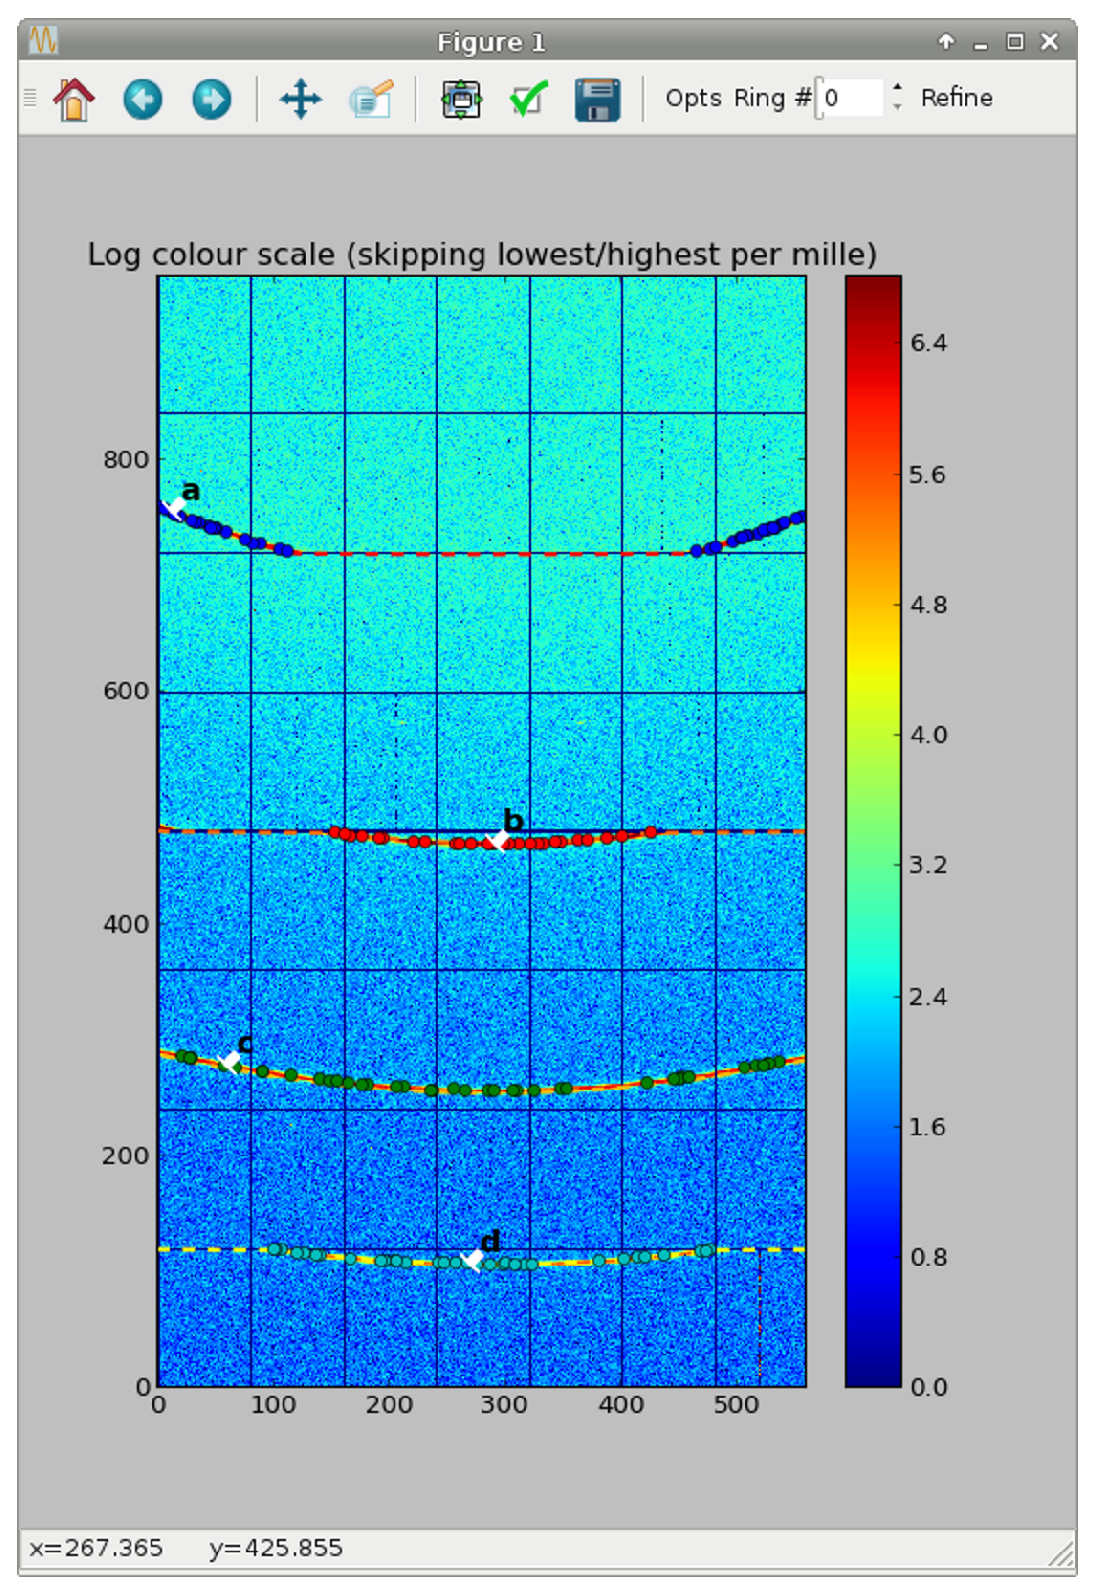
\includegraphics[width=9cm]{calib_xpad.eps}
\caption{The pyFAI calibration window: manual peak-picking and
ring assignment can be performed though it.
% The data correspond to a silver
% behenate sample, used as a calibrant on the BioSAXS beamline BM29 at the synchrotron ESRF
% (detector: Pilatus 1M, $\lambda=1.0${\AA})}
The data correspond to a lanthanum hexaboride (LaB$_6$) calibrant on the Cristal
beamline at synchrotron Soleil taken at 18.57 keV on a Xpad S540 flat pixel
detector tilted vertically by about 15$^o$.
This detector presents large (vertical) gaps between modules, explaining the
incomplete arcs of rings \textit{a, b} and \textit{d}.
Extracted control points are marked with dots, one color per group (assigned to
a letter) and the fitted iso-$2\theta$ contour are overlaid as dashed lines
(red, orange and yellow colored).
The iso-$2\theta$ contour plot is not smooth due to gaps in the
detector, explaining the incompleteness of some rings.}
\end{center}
\end{figure}

From this initial rough calibration on, pyFAI enables  the user to perform
many operations in the Command Line Interface (CLI) mode, like setting,
constraining, fixing and  refining parameters, extracting a new set of
key-points or performing the integration.
The complete set of options is described in appendix \ref{annex_calib}.

\section{Azimuthal Integration}

The core task of pyFAI, as the name suggests, is to perform 1D or 2D azimuthal
(and radial) integration as fast as possible. To achieve good performances in a
Python environment, several binary extensions are used to enable multi-threading
or even many-core acceleration (i.e. Graphics Processors Units (GPU) and Intel Xeon Phi
accelerators).
% And all this while offering a simple common interface at the Python level.
More details on the techniques used to speed up the code, especially on the GPU porting
are described in \cite{kieffer_ashiotis-proc-euroscipy-2014} and briefly
summarised in appendix \ref{annex_opencl}.

\subsection{Programming interface for azimuthal integration}

The initial idea behind pyFAI was to provide an easy way to perform
azimuthal/radial integration for scientists, ideally in a single command.
In the following snippet code we show how this is done:

%\begin{minted}{python}
\begin{verbatim}
import pyFAI, fabio, pylab
img = fabio.open("imagefile.tif").data
ai = pyFAI.load("geometry.poni")
tth, I = ai.integrate1d(img, 1000, unit="2th_deg", \
                        method="splitpixel")
pylab.plot(tth, I)
pylab.show()
\end{verbatim}
%\end{minted}

In the first line, three key libraries are loaded: fabio \cite{fabio} to read
images, matplotlib \cite{matplotlib} to display the results and pyFAI itself to
be able to perform azimuthal integration.
In the second and third line,  the image and the geometry are loaded.
The two last lines are meant to display the result.

In this snippet, the most crucial part is the fourth line, in which the image
\textit{img} is azimuthally integrated over 1000 bins with conversion  into
the output space which is the cone aperture ($2\theta$) given in degrees.
Other output units like the scattering vector $q$ or the radius $r$ (in the
detector plane) are available. By the \textit{method} keyword one can select the
algorithm to be used.

\subsection{Pixel splitting schemes and implementation}

PyFAI implements a dozen of azimuthal integration procedures which can be
classified according to the way the integration is performed and which pixel
splitting scheme is used (see table \ref{table_methods}).

\subsubsection{Histogram vs Look-Up Table.}
The naive way to integrate data (also called ``direct integration'') is to treat
an image pixel by pixel, very much like a histogram.
This is a \textit{scatter} operation which is hard to parallelize but cheap as
to memory occupation.
Using a \textit{scatter to gather} transformation, the azimuthal integration for
a given geometry can be stored into a look-up table (LUT) and applied like a
sparse-matrix-times-dense-vector multiplication (sometimes called
``backwards integration'').
Whilst being much more memory consuming, this
implementation is effective in terms of parallelization and speed.
The Compressed Row Storage (CSR) matrix representation is now used instead of
the LUT and generates a smaller memory footprint.

\subsubsection{Three pixel splitting schemes} are available in pyFAI and define
the way photons counted by a pixel are assigned to the various histogram bins,
especially when the pixels are large (like on Pilatus detectors):
\begin{itemize}
\item No splitting: the full intensity is assigned into a single bin (Dirac
like shape), the one at the middle of the pixel (like in the histogram).
\item Bounding box splitting: the pixel is abstracted by a simpler rectangular box
oriented parallel to the radial and azimuthal directions
\item
Tight/full pixel splitting: the only assumption made is that pixel
edges deemed to be straight lines. This is also known as polygon based
interpolation \cite{stefanvdw}.
\end{itemize}
Figure \ref{split} Displays the way a single pixel is split into a
large number of bins using the three schemes explained above.
The way FIT2D splits pixels has been added for comparison: it looks
similar to the bounding box pixel splitting but there are differences
in the implementation details.

\begin{figure}
\label{split}
\begin{center}
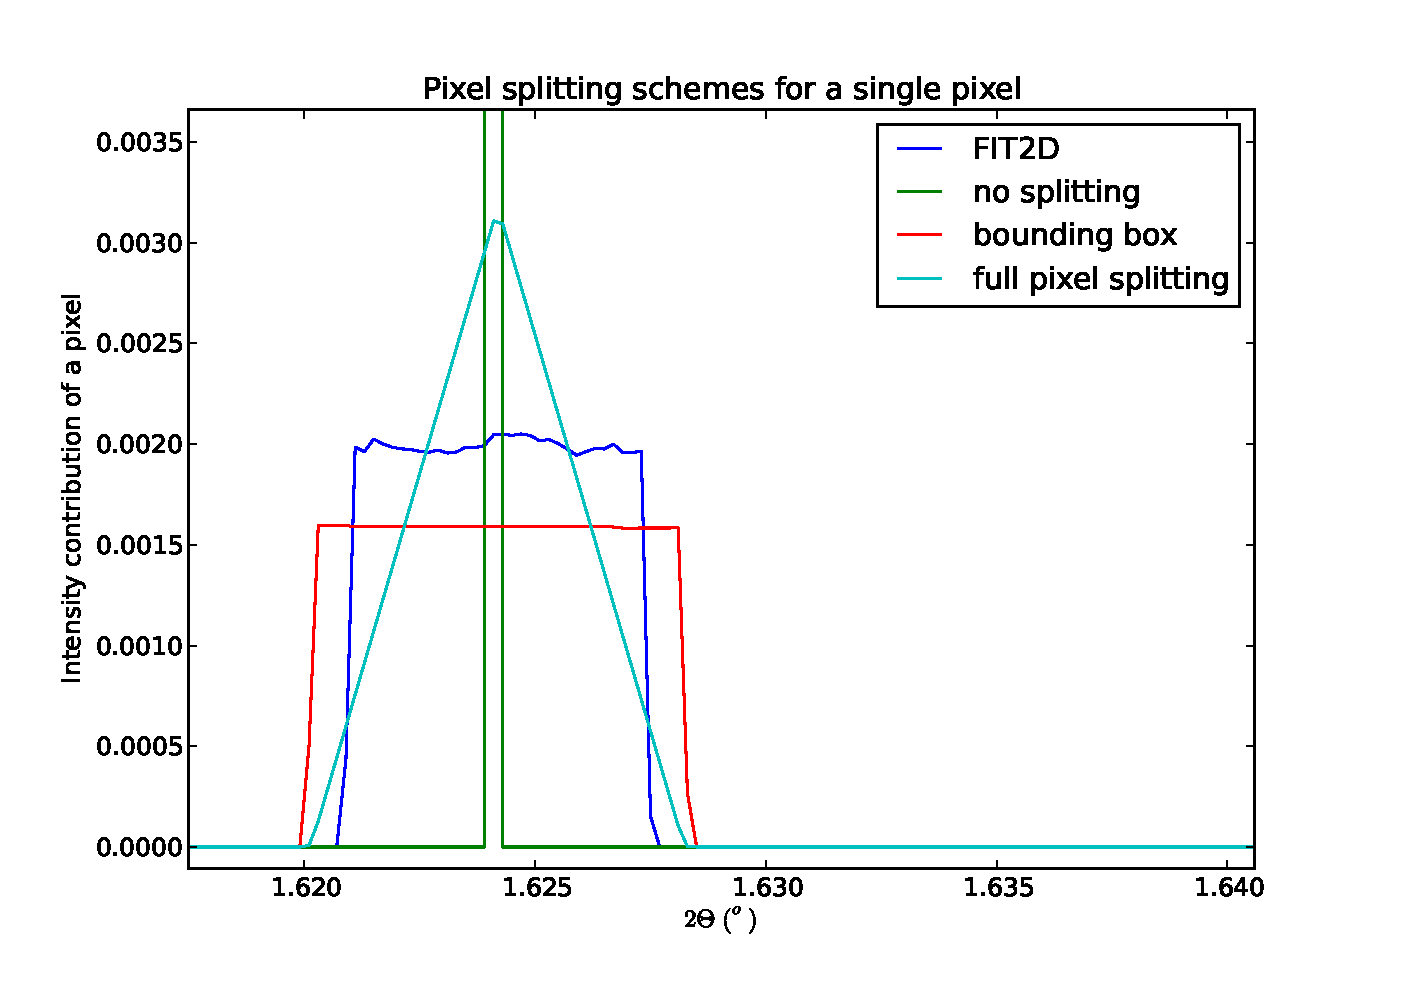
\includegraphics[width=9cm]{splitpixel.eps}
\caption{Contribution to a powder diffraction pattern from a single pixel
showcasing the different pixel splitting algorithms. PyFAI implementations are
compared to the FIT2D corresponding algorithm.}
\end{center}
\end{figure}

\subsubsection{Speed and memory consumption.}

The table \ref{table_methods}  lists the various available implementations
together with their execution speed and the memory footprint for integrating a 2048x2048
pixel image into 1000 bins.

\begin{table}
\label{table_methods}
\caption{Methods available within pyFAI for azimuthal integration
along with their speed and memory footprint. 
Measurements were performed on a 3 GHz quad-core
computer using a 2048x2048 pixel image.}
\begin{tabular}[pos]{c|c|c|c}
%\begin{tabular}[pos]{|c|l|l|l|}
%\hline
Pixel splitting			& Direct histogram 		& Look-up table (reverse) \\
\hline
No splitting          & numpy (889ms 336MB)  &CSR nosplit (48ms 330 MB)\\ 
					  & cython (361ms 323 MB) & \\
\hline
Bounding box          & splitbbox (129ms 343MB) & splitBBoxLUT (59ms 327MB)\\
					&						&	CSR bbox (52ms 330MB) \\
\hline
Tight splitting & splitpixel (516ms, 480MB) &CSR full (51ms, 502MB)\\
%\hline
\end{tabular}
\end{table}


\subsubsection{About error propagation:}
during the regrouping process, pyFAI can propagate errors, assuming that the
initial pixel-wise variance is known, for example as extracted from a
multi-frame experiment. Beside this, two single-frame variance estimators are
available: the Poisson model assumes that the variance within a pixel equals to
the raw signal and propagates it. The second estimator postulates the
isotropic distribution of the signal and calculates the variance within all
pixels contributing to a single output bin. 

While pixel splitting provides smoother
results, any pixel splitting scheme introduces some serial correlation between
neighbouring bins, resulting in an overestimation of the propagated error,
as described in \cite{billinge2014}. 
Nevertheless, this effect is often negligible due to the point-spread function
of typical area detectors.

\subsection{Graphical user interface for azimuthal integration}

A minimalistic GUI called \textit{pyFAI-integrate}, is
shown in figure \ref{pyFAI-integrate}.
It illustrates most of the feature available in pyFAI:
the top frame displays the geometric description of the experiment.
The middle frame targets the per-pixel corrections to be applied: dark current
subtraction, flat-field correction, polarisation and solid angle effects, static
and dynamic masking. The check boxes next to each field are used to toggle the given correction.
The third frame displays information about the output format, the
number of bins in radial and azimuthal directions together with the
selection of the integration output space (these are mandatory).
The bottom frame allows an OpenCL device (CPU/GPU) to be selected for use in
the computation.

\begin{figure}
\label{pyFAI-integrate}
\begin{center}
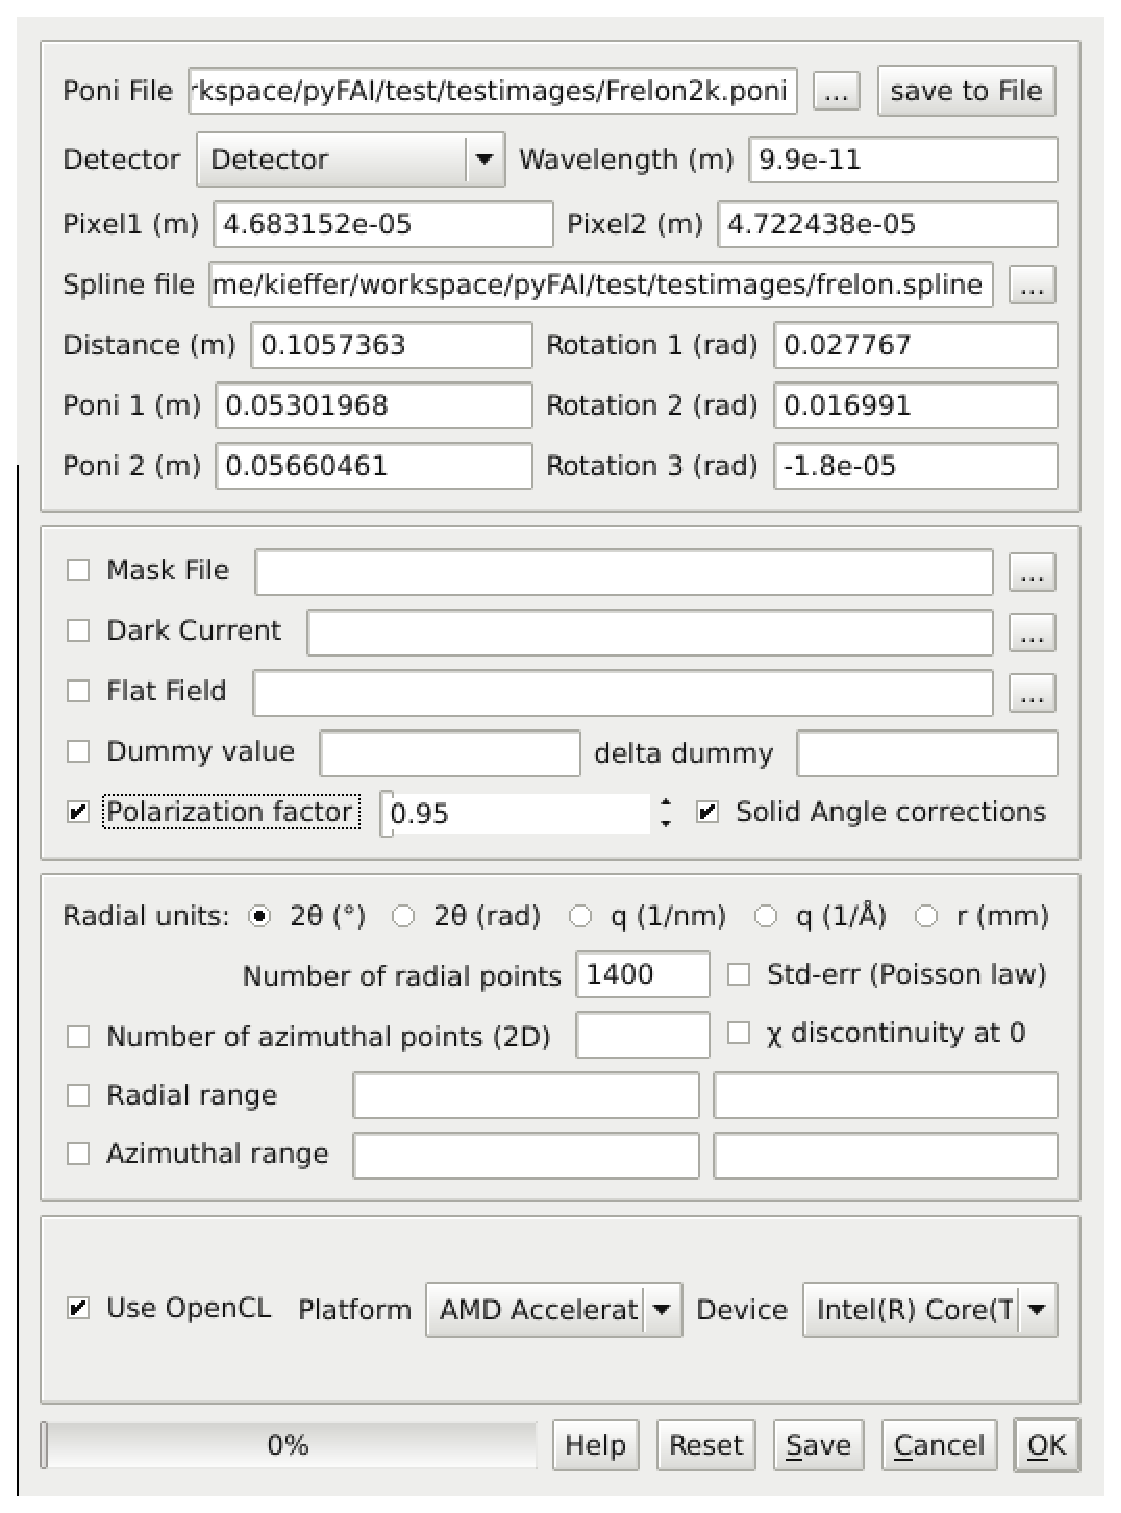
\includegraphics[width=9cm]{integrate.eps}
\caption{Graphical interface for performing azimuthal integration on a set of
images.}
\end{center}
\end{figure}

\section{Application Examples}

Azimuthal regrouping and its inverse transformation (assuming
uniform intensity distribution throughout the azimuthal angles) can be performed
using pyFAI, which offers many opportunities for applications.

\subsection{Diffraction image generation}

Once the geometry has been defined (i.e. by loading a \textit{PONI-file}), the
$2\theta$ and $\chi$ positions of every single pixel of the detector are known.
If one assumes signal isotropy along the azimuthal angle range (like an
ideal powder without preferred orientation), \textit{2D} diffraction patterns can be
generated as illustrated in the example below:

%\begin{minted}{python}
\begin{verbatim}
import numpy, scipy.signal, pyFAI
N = 1000 
tth = numpy.linspace(0, 60, N)
# generate the powder curve as a single Gaussian
I = scipy.signal.gaussian(N, 5)
det = pyFAI.detectors.detector_factory("Pilatus1M")
ai = pyFAI.AzimuthalIntegrator(dist=0.1, poni1=0.1,\
                             poni2=0.1, detector=det)
img = ai.calcfrom1d(tth, I)
\end{verbatim}
%\end{minted}


The method \textit{calcfrom1d} is available from any
\textit{AzimuthalIntegrator} or \textit{Geometry} class instance.
It is used together with a calibrant object to simulate a diffraction
image suitable to test pyFAI or other calibration codes (for example to
validate the geometry transformation from one program to another).



%\begin{minted}{python}
\begin{verbatim}
import pyFAI.calibrant
lab6 = pyFAI.calibrant.ALL_CALIBRANTS["LaB6"]
lab6.set_wavelength(1e-10)
img_lab6 = lab6.fake_calibration_image(ai)
\end{verbatim}
%\end{minted}

In the above code snippet, second line, a reference sample,
LaB$_6$, is chosen from the list of calibrants known to pyFAI before the
wavelength is set.
Once combined with the geometric information, the \textit{calibrant} object is
able to generate a 2D \textit{numpy} array containing the simulated Debye-Scherrer
diffraction rings which can be saved or displayed on the screen.
The \textit{fake\_calibration\_image} method takes more parameters to help set
the U, V and W parameters from Caglioti's formula \cite{caglioti} to include the
broadening of peaks according to the simple resolution function.
In pyFAI, only the \textit{d-spacing} values of the calibrants are stored, thus
the reconstructed image will have all rings with the same intensity (once integrated).

\subsection{Image offset and validation of the calibration}
By regenerating a 2D diffraction image from the integrated powder pattern one
can assess the quality of the calibration used for the integration.
The calibration tool, \textit{pyFAI-calib}, includes  a ``validate'' command
which evaluates the spatial offset between the 2D diffraction image and the
image regenerated from the integrated pattern, using a classical phase
correlation algorithm.
This detemines the precision of the PONI localization, which
can be better than a tenth of a pixel, when calibrating images with continuous
rings (i.e. not spotty) and with a mask large enough to remove the beam stop and
all parasitic scattering.

\subsection{Amorphous background removal}

The pyFAI azimuthal integrator features a \textit{separate} method for
separating automatically a background featuring an azimuthal symmetry
(amorphous scattering or powder ring), from the Bragg peaks.

Based on what was described in \cite{PyFAI_PDJ}, \textit{2D-}azimuthal
integration is performed on the input image.
The output 2D image is filtered along the azimuthal $\chi$ axis using a
percentile (often the median) filter to reconstruct the powder diffraction curve
without the sharp Bragg spots.
The number of points in azimuthal and radial direction as well as
the percentile value can be adjusted but the default values are in
general reasonably good.

The reconstructed 2D image corresponds to the amorphous/powder/isotropic
component of the input image and the subtraction of this image from
the raw data contains only the signal coming from large crystals.
Figure \ref{separate} (left hand side)
presents a close-up of protein single crystal data recorded on a Pilatus3-2M
detector (image taken at the ID23-2 beamline of the ESRF).
A diffuse amorphous halo is clearly visible.
After using the automatic amorphous background removal, which takes into account
the mask needed for such pixel detectors, only Bragg peaks remain (right hand
side of the image).

\begin{figure}
\label{separate}
\begin{center}
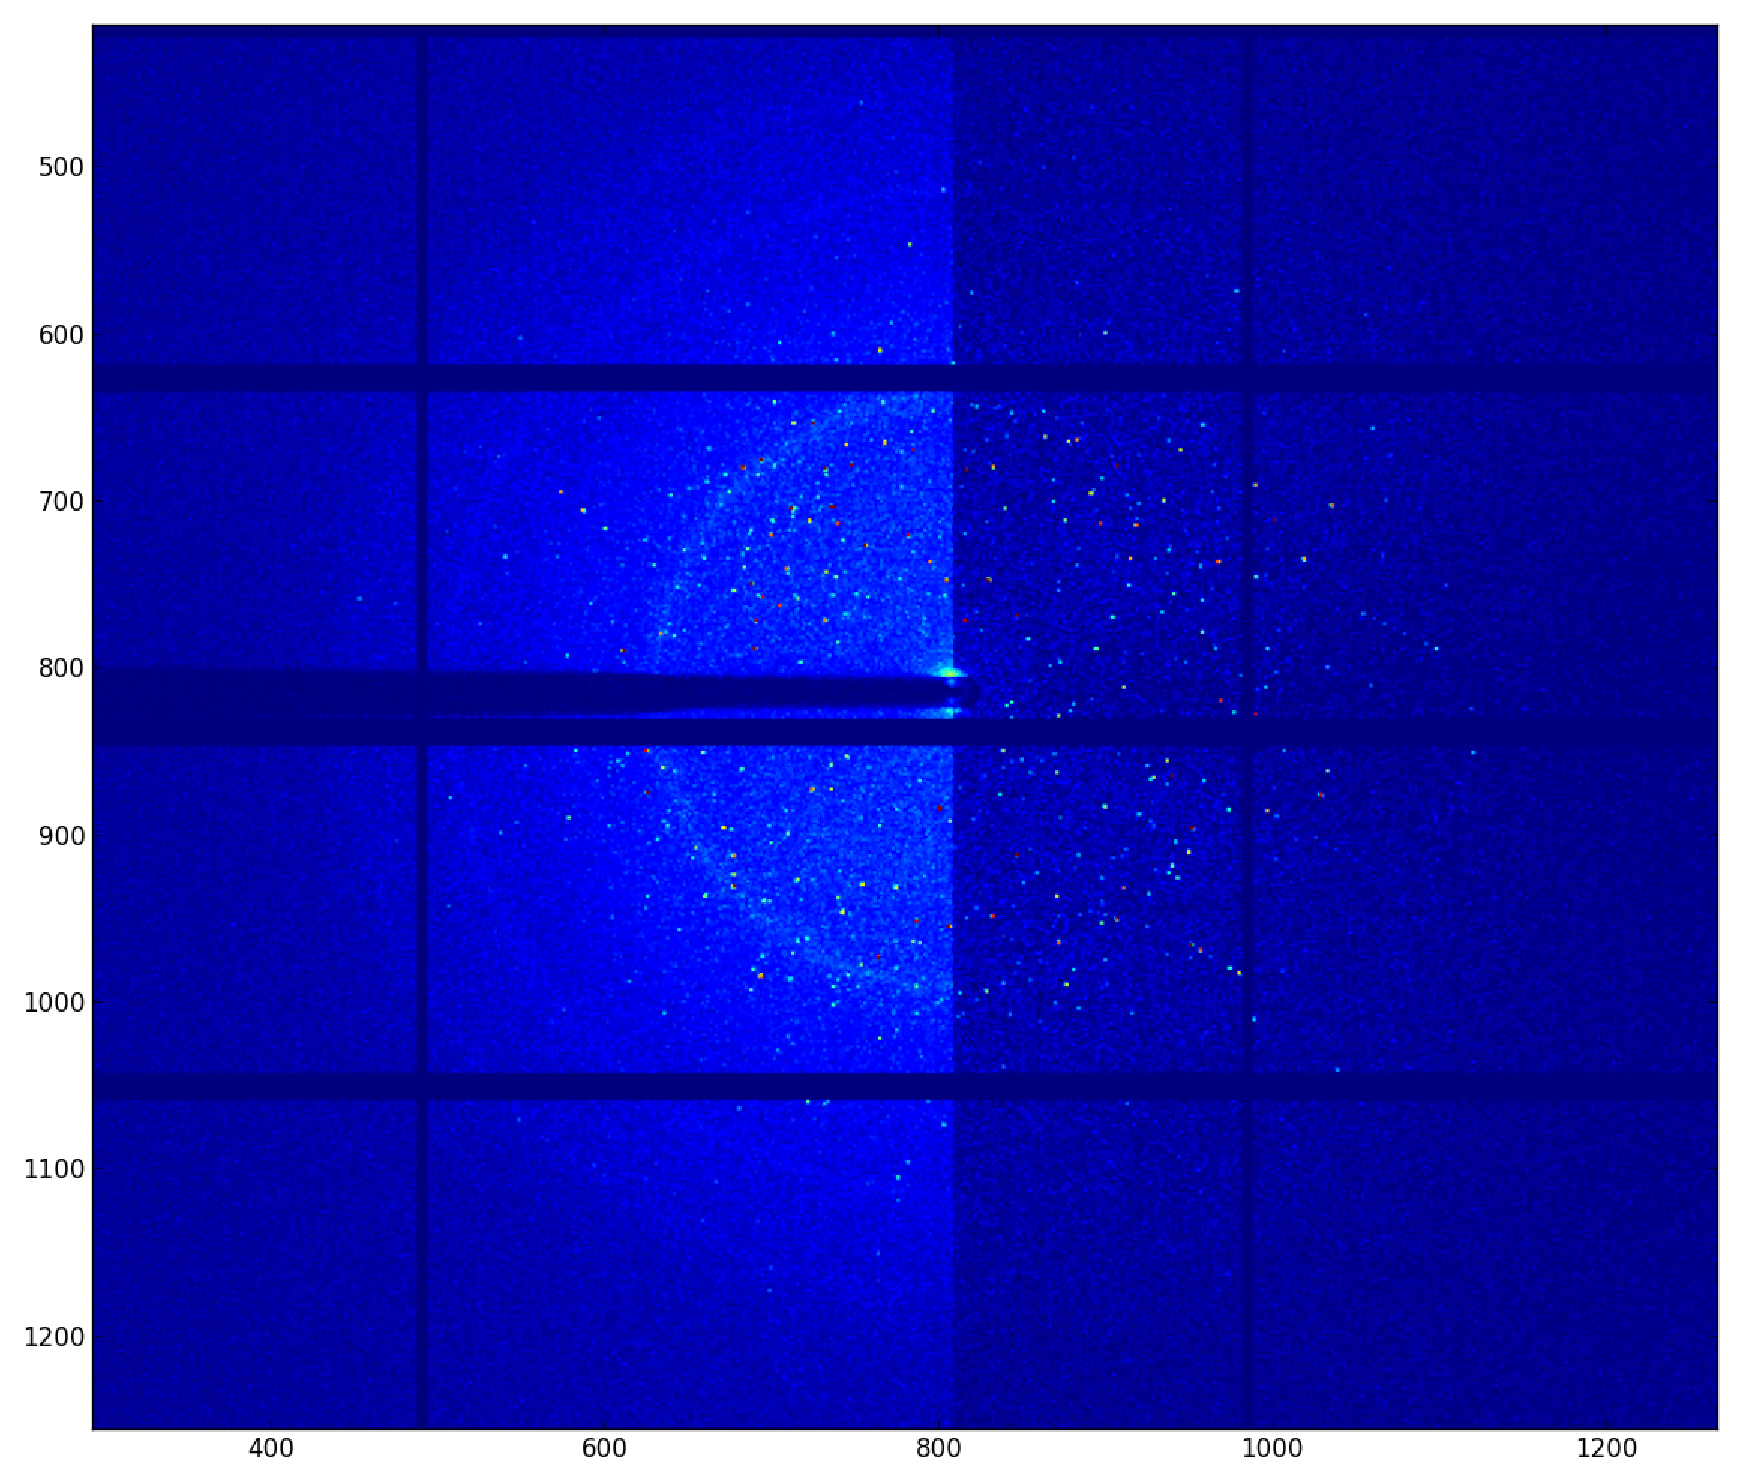
\includegraphics[width=9cm]{separate_id23.eps}
\caption{Automatic removal of the amorphous signal (ice ring) from Bragg peaks
in a protein crystallography experiment (data from the beamline ID23-2 at
the ESRF).}
\end{center}
\end{figure}

\subsubsection{Application to serial crystallography:}
In serial crystallography experiments, tiny crystals in their solvent are moved
into the X-ray beam (using a jet or moving a sample holder) and scattering
data are acquired continuously, using a fast detector (from dozens of Hz to kHz).
These experiments produce a huge amount of data while only a small fraction of the
frames contain some diffraction signal.
PyFAI has been integrated into the processing software \textit{NanoPeakCell}
which provides a graphical interface for frame selection in serial crystallography.
PyFAI has also been integrated into the LImA data acquisition system
\cite{lima}, where the amount of single crystal diffraction data within each
frame can be assessed and a decision taken whether to save a given frame or
not.
This way, a huge amount of disk space and network bandwidth
can be saved.

\section{Related Work}

Currently, the pyFAI library runs either as stand-alone application or
embedded in other software on several beamlines at the ESRF to
perform azimuthal/radial integration on-line:
\begin{itemize}
  \item inside the LImA image acquisition library, running on the
  computer controlling the camera,
  \item in one dedicated data-analysis server like EDNA \cite{edna} in the case
  of the BioSaxs beamline, BM29 \cite{bm29} or the Dahu server at the TRUSAXS
  beamline, ID02.
\end{itemize}

Other institutes have independently integrated pyFAI into their processing
pipelines: \textit{NanoPeakCell} (developed at IBS by N. Coquelle),
\textit{PySAXS} (developed at CEA by O. Taché), \textit{Dpdak} (developed
at the Petra III synchrotron by G. Benecke and co-workers) \cite{dpdak}
and \textit{Dioptas} (developed at the APS synchrotron by C. Prescher).
Most of these software packages offer a GUI to facilitate the
data processing for a specific type of experiment.

\section{Conclusion and Future Work}

In this work, we have described the improvements in the
v0.10 of the pyFAI library, focusing on the detector representation in space, ring
extraction algorithms and pixel splitting schemes for azimuthal integration.
The number of independent projects relying now on pyFAI proves that it fulfills a
number of needs in the scientific community.

On the other hand, there are plenty of unresolved issues: all
algorithms designed to perform azimuthal integration are not yet implemented in
2D. Is it possible to address the error propagation issue while keeping pixel
splitting? Can all algorithms used in pyFAI be ported to GPU to off-load the
processor? The GUIs for calibration and integration, while helpful, are really
minimalistic.
The automatic ring extraction using \textit{computer vision} techniques can
be improved and the calibration might be fully automated.
The functionality relating to the geometry refinement of non planar
detectors is not yet complete.
%This summarizes well the work already done and gives an
%outlook for forthcoming features.
The version number (v0.10) clearly indicates that a great
wealth of work has been done but also yields a warning about possible changes
in the programming interface in future versions for encompassing numerous new
features.
The open source nature of the project means that such changes will be 
fully visible and is intended to encourage contributions from the community.


\bibliographystyle{iucr}
\bibliography{biblio}
\appendix
\section{Project structure}

PyFAI is an open source project licensed under the General Public License (GPL
v3+).
It is mainly written in Python (v2.6, 2.7, 3.2 or newer) and is
heavily relying on the Python scientific ``ecosystem'': NumPy \cite{numpy}, 
SciPy \cite{scipy} and Matplotlib \cite{matplotlib}.
It exhibits high performance in image treatment and azimuthal/radial integration
thanks to Cython \cite{cython} and PyOpenCL \cite{pyopencl}.
PyOpenCL remains an optional dependency, therefore all OpenCL code features a
Python or Cython implementation as well.
For sake of consistency with other ESRF software projects \cite{pymca}, the
GUI was developed using PyQt (or PySide).
The project is hosted on GitHub (\textit{https://github.com/pyFAI}) which
provides the issue tracker in addition to code hosting.
A pyFAI mailing list is
available: \textit{pyfai@esrf.fr} (send ``subscribe pyfai'' by e-mail to
\textit{sympa@esrf.fr} to subscribe to the mailing list). New features
and changes in the API are disscussed there.

Originally developed under Linux, the software is also tested and supported on
other operating systems like Windows and MacOSX.
To ease the distribution, the software is available on the PyPI package
repository (\textit{http://pypi.python.org}) and as official Debian package and
included in other well-known Linux distributions like Ubuntu.

Everyone is welcome to fork the project and adapt it to his/her own needs:
CEA Saclay, Soleil, DESY and APS have already done so.
Collaboration is encouraged and new developments can be submitted and merged
into the main branch via pull-requests (on the github interface).

While there are a couple of official releases every year (better
tested versions), pyFAI features a comprehensive test suite and uses
\textit{continuous integration} mechanism to ensure that any snapshot of the
master branch provides \textit{valid} results.

\section{Calibration tool}
\label{annex_calib}

The pyFAI calibration tool, called \textit{pyFAI-calib}, has been available
along with the integration tool since the very beginning of the project, 
since having the same geometry module for both calibration and integration 
has been a top priority in the project's specifications.
The geometry file (commonly called \textit{PONI-file}) is updated at each
optimization step and delivers the whole description of the experiment
(together with time-stamps, making it easy to edit by hand).
This single-file geometry avoids copy-and-paste errors of spatial coordinates.

\subsection{Calibration command line interface}

While the GUI for peak-picking has significantly improved
(figure \ref{calib}), the command line interface used for the optimization
process has become more versatile.

Starting from an initial, coarse calibration, pyFAI allows performing many
operations to refine all parameters: distance, centre position, rotation of
the detector and, optionally, the wavelength (all units are in the S.I).
The available commands are:
\begin{itemize}
\item \textit{help}: shows the help message
\item \textit{abort}: quits the program directly
\item \textit{assign}: changes the assignment of groups to rings
\item \textit{done}: performs the azimuthal integration and quits
\item \textit{get}: prints out the value of the requested parameter, \\
	\verb|get wavelength|
\item \textit{set}: defines the value of the selected parameter,\\
	\verb|set wavelength 1.54e-10|
\item \textit{bound}: selects the region of validity for a given parameter,\\
	\verb|bound dist 0.1 0.5|
\item \textit{bounds}: reviews and modifies the region of validity for all
parameters
\item \textit{fix}: prevents the parameter from being refined,\\
	\verb|fix wavelength|
\item \textit{free}: allows the parameter to be refined,\\ 
	\verb|free rot1|
\item \textit{refine}: re-runs the least squares refinement
\item \textit{validate}: estimates the accuracy of the calibration on
the whole image by overlaying and correlating the raw image with the
back-projected integrated pattern
\item \textit{recalib n blob}: extracts a new set of control points from the
\textit{n} innermost rings. The optional parameter \textit{blob}
selects the ring extraction algorithm to use.
\item \textit{reset}: sets the geometry to its default values (centred
orthogonal detector)
\item \textit{show}: prints out the current geometry parameters on the screen
\item \textit{integrate}: performs the 1D and 2D integration and displays it in
a separate window to validate the quality of the calibration.
\end{itemize}

If the initial calibration is correct, like in figure \ref{calib}, the procedure
to get a perfect calibration should be ``\textit{recalib}$\hookleftarrow $
\textit{done}$\hookleftarrow \hookleftarrow $''.
If the predicted rings become too large or too small compared
to the actual ones, the wavelength can be refined.
For this purpose, it is advisable to  extract as many rings as
deemed reasonable using \textit{``recalib n''} then run \textit{``free wavelength''} and
\textit{``refine"}.% to check if there's an improvement.
Since distance and wavelength are
heavily correlated, it is important to take into account as many rings as
possible at high angle.

The \textit{validate} option allows measuring the offset between the actual
diffraction image and an image generated from the refined geometry using phase
correlation.
In most cases it is possible to attain a precision of about one tenth of a pixel
for determining the PONI position.

\subsection{Automatic distance and centre calibration}
The calibration procedure has been automated for the  Macromolecular
Crystallography beamlines (MX) at the ESRF.
The sample-to-detector distance and the beam centre need to be inputted in the
header of the collected images in order to process them automatically.
As the area detector is on a moving stage, distance and centre position are
changing at every data collection.
Via the \textit{MX-calibrate} tool of pyFAI, it is possible to calibrate the
geometries of a set of images recorded at various distances using Debye-Scherrer
rings of a reference compound.
After performing subsequently the peak-picking using \textit{blob-detection}
(as described in \ref{blob}) and the least squares refinement of the geometry on
every input frame, distances and beam centre positions are returned as function
of the detector motor position, without manual intervention.

\section{Layers in pyFAI library}
PyFAI has multiple
entry-points depending on the type of application and the user skills.

\subsection{Top level graphical application}
A couple of top level applications: \textit{pyFAI-calib} and
\textit{pyFAI-integrate} provide a graphical user interface to inexperienced
users. 
These interfaces are the least flexible ones and, bacause they are
GUIs, are not tested against regression.

\subsection{Top level application}
A bunch of simple scripts are provided with pyFAI for various kinds of
processing (like \textit{pyFAI-saxs},  \textit{pyFAI-waxs} and also \textit{diff\_tomo}) 
which can be integrated into shell scripts for batch
processing. 

\subsection{Top level Python interface}
PyFAI provides at the top level the AzimuthalIntegrator object which can be
created from a \textit{PONI} file and used to integrate data. 
Pre-processing options
(dark, flat, mask, solid angle and polarisation correction) can be passed to
the \textit{integrate1d} or \textit{integrate2d} methods.
These methods also ``know'' how to save processed data on disk.
This is probably the most flexible level of use of pyFAI, and the best tested
one. Moreover nothing from the underlying levels is hidden.

\subsection{Mid level API}
Below the AzimuthalIntegrator are the geometry calculation, the detector
description, calibrants, geometry refinement \ldots 
These module are
implemented in Python using NumPy but often, a second
implementation exists in Cython for performance purposes.
The equivalence of these implementation is a core target of the pyFAI test
suite

\subsection{Regridding/histogramming engines}
These number-crunching engines are typically written in Cython or OpenCL with a
Python binding and can only be accessed from the Python level. 
They expose only the core number crunching routines for integration or
distortion correction.

The pyFAI project is very modular and can be accessed at various
levels depending on the user's needs.

\section{Parallel implementations using OpenCL}
\label{annex_opencl}
Azimuthal integration, like  many computationally intensive parts in pyFAI,
was written as OpenCL kernel and interfaced to Python via PyOpenCL
\cite{pyopencl}.
PyOpenCL provides a shared execution model which is effective both on
usual processors (CPU), graphics cards (GPU) and accelerators like the Intel
Xeon Phi.

\subsection{Azimuthal Integration}
The direct azimuthal integration (histogram) is basically a scatter operation
which requires extensive memory locking (inefficient over many threads).
To overcome this limitation, pixels have been
associated to the output bin of the histogram and stored in a look-up
table (LUT), making the integration look like a simple (if large and sparse)
matrix-vector product \cite{PyFAI_PDJ}.
The sparse matrix ``Compressed Row Storage'' (CSR) format is now used in pyFAI,
using only half of the space that the LUT previously used \cite{kieffer_ashiotis-proc-euroscipy-2014}.
Furthermore, all threads within a workgroup are collaborating to calculate the
matrix-vector product via a so-called ``parallel reduction'', ensuring
additional speed-up (especially on GPUs).
The compensated algebra (Kahan summation) is kept to maintain the accuracy
of the calculation while using single precision (32 bits) floating point
arithmetic.

\subsection{Performances}
Figure \ref{benchmark} shows the performance of pyFAI in terms of frames
processed per second versus the input image size (in semi-logarithmic scale).
The computations were run on a dual socket Intel Xeon
E5-2667 (2 hexacore @2.9Ghz) computer with a Nvidia Tesla K20 GPU and an Intel
Xeon Phi accelerator.

\begin{figure}
\label{benchmark}
\begin{center}
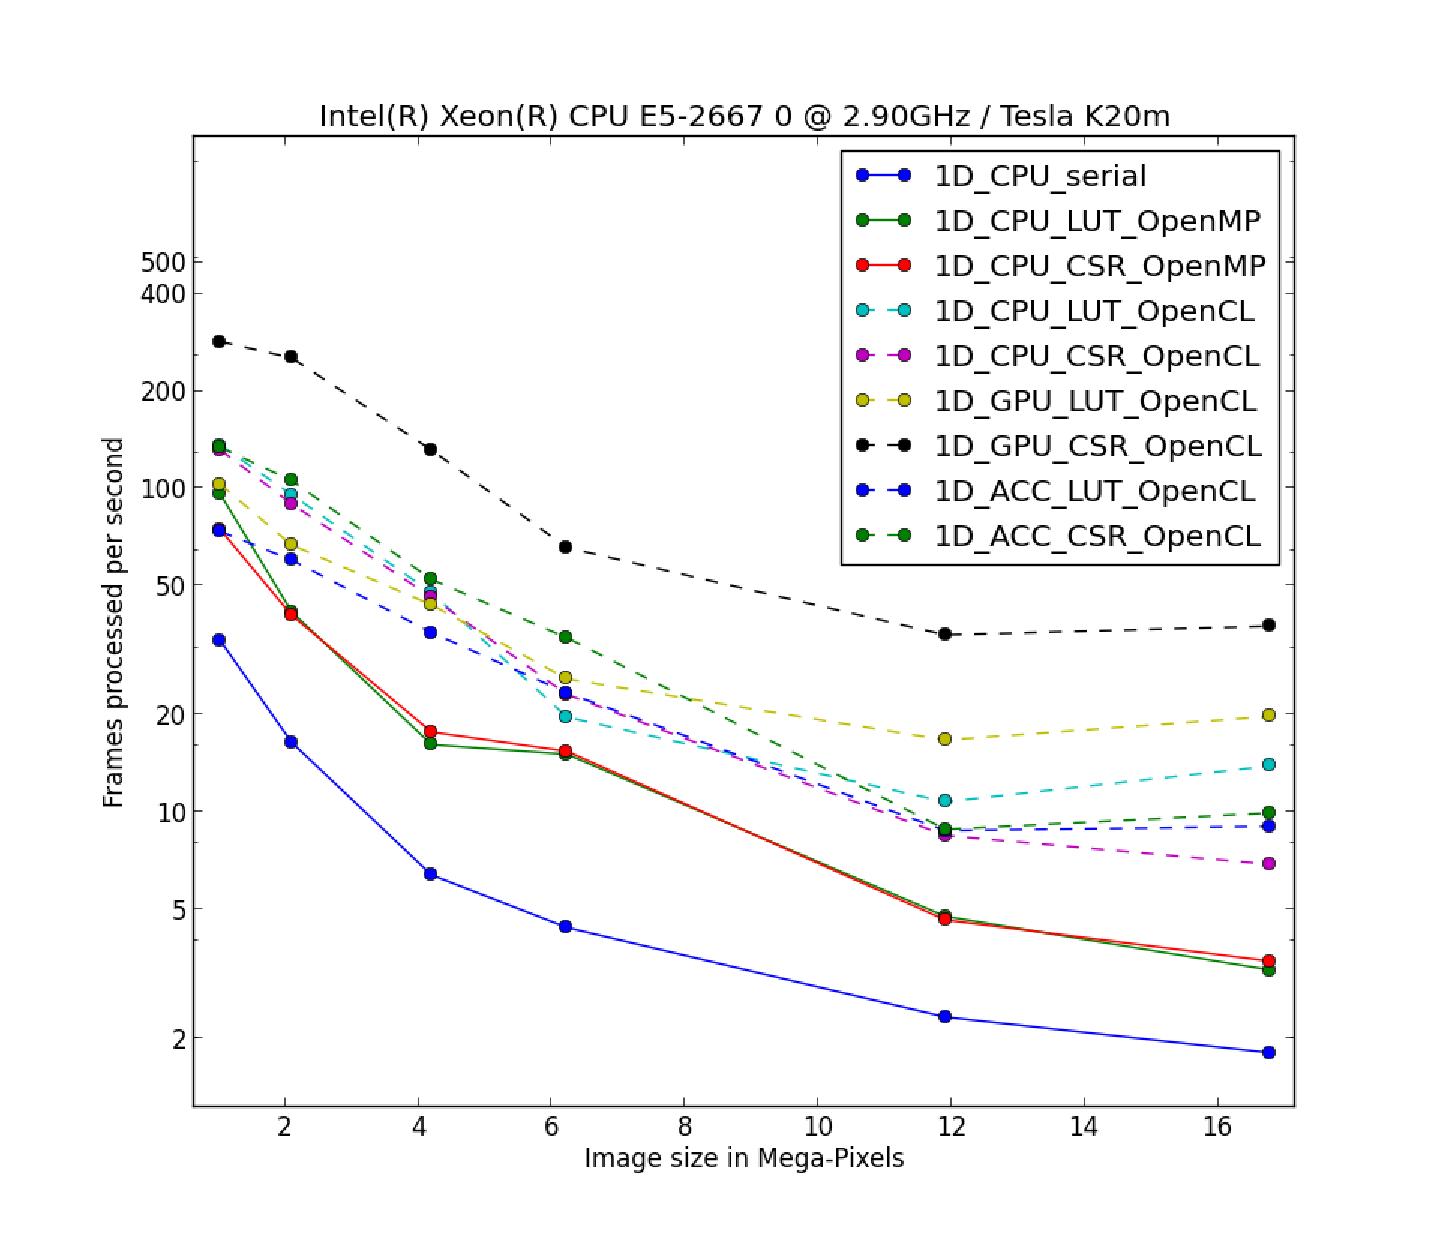
\includegraphics[width=9cm]{benchmark.eps}
\caption{Comparison between the various pyFAI algorithms performing
azimuthal integration}
\end{center}
\end{figure}

In this benchmark, four groups of curves can be identified:
\begin{itemize}
  \item The lower continuous blue curve presenting the serial Cython code using
  histograms (corresponding to the ``splitbbox'' method) which is the slowest
  implementation (even if it is 7x faster than a numpy implementation).
  \item The red and green continuous curves which correspond to the two parallel
  Cython implementations for look-up-table-based integration (using LUT and CSR
  representation).
  \item The group of dashed curves which represent the OpenCL optimised code
  running on 12 CPU cores, 60 cores from the accelerator, and GPU (LUT
  implementation), respectively.
  \item The upper dashed black curve, hence the fastest, corresponds to the CSR
  sparse matrix multiplication algorithm implemented in OpenCL and runs on
  the Tesla K20 card.
  It is twice faster than any other implementation: a 4096x4096 pixel
  image can be processed in less the 19 milliseconds, i.e. 885 Mega-pixels
  per second.
  This gain in performance is obtained from the collaborative
  partial reduction of all threads within a workgroup.
\end{itemize}


\ack{Acknowledgements}

We would like to thank all ESRF beamline teams for supporting the
pyFAI development, especially BM01, BM02, ID02, ID11, ID13, ID15, ID21, ID23,
BM26, ID29, BM29 and ID30.
In the instrumentation division (ISDD) we would like to thank Claudio
Ferrero, head of data analysis unit, for the critical revision of this
manuscript and Andy G\"otz, head of software group, for supporting the
algorithmic work performed on pyFAI in addition to the features exposed to the
user.
V. Armando Solé, the author of PyMca, is also acknowledged for delivering us
some crucial GUI building blocks.

The huge parallelisation work on the integration routines and their porting to
many-core devices was mainly done by Dimitris Karkoulis, Zubair Nawaz and Giannis Ashiotis,
thanks to the EU-grant LinkSCEEM-2 (RI-261600).

We would like to thank 
Erik Elka\"im from the Cristal beamline at Soleil for
providing the Xpad
%Martha Brennich for providing the silver behenate
calibration image (fig. \ref{calib}) and David Flot from beamline ID23 at
the ESRF for the protein diffraction image with ice-rings (fig.
\ref{separate}).
Finally we would like to thank our reviewers, especially Brian R. Pauw, for
their very constructive comments which helped us improve this article. 
\end{document}
